\documentclass{article}
\usepackage{graphicx} 
\usepackage{kotex}
\usepackage{listings}
\usepackage{float}

\usepackage[utf8]{inputenc}
\usepackage{listings}
\usepackage{xcolor}

\lstset{
  basicstyle=\ttfamily\small,
  keywordstyle=\color{blue},
  commentstyle=\color{gray},
  stringstyle=\color{red},
  showstringspaces=false,
  columns=fullflexible,
  keepspaces=true,
  language=Lisp,
  morecomment=[l]{;}
}


\title{프로그래밍 언어 HW4 제출}
\author{C335186 서장훈}
\date{2025.6.18}

\begin{document}

\maketitle


\section{Prolog 에 관해 공부한 내용 + 어려웠던 점}

Prolog는 명령형 언어처럼 변수를 선언하고 반복문을 돌리고 조건문을 쓰는 방식이 아니다. 사실과 규칙을 기반으로 추론하는 논리 프로그래밍 언어이다. 따라서 처음 접해봤을 때 어려움이 많았다. 평소 하던 코딩은 규칙에 맞춰 말하느 느낌이라면 Prolog는 수학식을 쓰는 느낌을 많이 받았다. \\ \\
Prolog는 1970대 논리학 기반으로 만들어졌으며 PROgramming in LOGic이라는 뜻이서 왔다고 한다. 
Prolog의 기본 개념은 동일화이다 이건 두 항을 비교해서 일치 가능한지 검사하고 가능하다면 변수에 값을 할당하는 과정이다. 예를 들어 parent(X, mary)와 parent(john, mary)는 동일화를 통해 X에 john을 할당할 수 있다. 이런 식으로 Prolog는 규칙을 체계적으로 적용해가며 추론을 진행한다. \\ \\
만약 실패가 발생한다면 Prolog는 백트래킹을 수행할 수 있다. 한 경로를 시도하다가 실패하면 이전 선택 지점으로 돌아가서 다른 가능성을 시도하는 것이다. trace를 켜서 call, exit, fail, redo 상태를 추적하여 이 흐름을 알아낼 수 있다. \\ \\
실습 중에 가장 많이 시간이 걸리고 어려웠던 것은 trace였다. insertion sort를 trace로 따라가면서 재귀가 어떻게 진행되고, 삽입이 어떻게 이뤄지는지 살펴봤다. 
특히 N-Queen 문제에서는 permutation을 이용해 가능한 모든 배치를 만들어서, safe\_all이라는 검사를 통해 대각선 충돌 여부를 확인했다. 
이 과정에서 trace를 통해 재귀 깊이가 어떻게 증가하고 백트래킹이 언제 발생하는지 명확히 볼 수 있었다. 
예를 들어 N=3에서는 모든 경우가 실패로 끝나는데, 이걸 trace를 보면 왜 그런지 과정 전체를 확인할 수 있다. \\ \\
그리고 특히 Prolog에서는 리스트가 매우 중요한 데이터 구조로 등장한다. 리스트는 atom, 변수, 숫자 등을 묶어서 대괄호 [ ]로 표현한다
. 예를 들어 [1, two, 'THREE', A] 같은 리스트를 만들 수 있으며, 리스트 안에 다시 리스트를 포함할 수도 있다 ([1, 2, [4, 5]]처럼). 리스트의 첫 원소와 나머지를 구분할 때 Head | Rest 표기법을 사용하는데, 이 구조를 이용한 재귀적인 리스트 처리 코드가 매우 자주 등장한다. \\ \\




\newpage
\section{hw5a.pl}
\subsection{hw5a.pl 코드}
\begin{lstlisting}

% Main entry point: sort List into Sorted
sorting(List, Sorted) :-
    insertion_sort(List, Sorted, 0).  % Start with recursion depth 0

% Insertion sort with recursion depth tracking
insertion_sort([], [], _).  % Base case: empty list is already sorted
insertion_sort([H|T], Sorted, D) :-
    D1 is D + 1,  % Increment recursion depth
    insertion_sort(T, SortedTail, D1),  % Recursively sort tail first
    insert(H, SortedTail, Sorted),  % Insert current head into sorted tail
    ( D > 0 -> print_X(Sorted) ; true ).  % Print intermediate results only if depth > 0

% Insert element X into a sorted list
insert(X, [], [X]).  % Insert into empty list
insert(X, [H|T], [X,H|T]) :- X =< H.  % Insert before first larger element
insert(X, [H|T], [H|R]) :- X > H, insert(X, T, R).  % Recurse until correct position found

% Print the current state of the list
print_X(List) :-
    write('X = '),
    print_list(List).

% Print list with pretty formatting
print_list([]) :- write('[]'), nl.
print_list([H|T]) :-
    write('['), write(H), print_tail(T).

% Continue printing the rest of the list elements after the first one
print_tail([]) :- write(']'), nl.
print_tail([H|T]) :-
    write(', '), write(H), print_tail(T).

\end{lstlisting}


\subsection{hw5a.pl 코드 설명 (trace 사용)}
\begin{figure} [H]
    \centering
    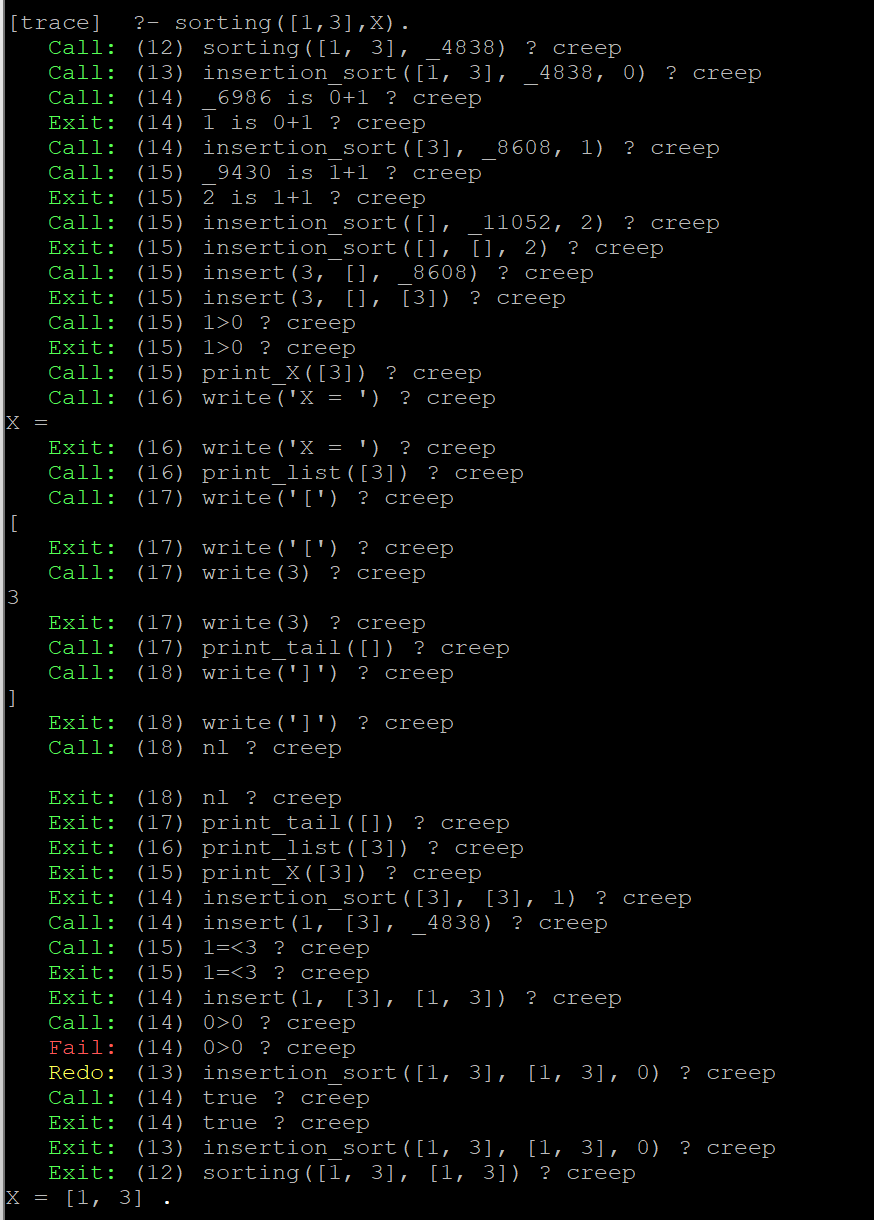
\includegraphics[width=1\linewidth]{trace1.png}
    \caption{Enter Caption}
    \label{fig:enter-label}
\end{figure}

우선 trace를 통해 코드 구조를 설명하기 위해 trace 결과를 가져왔다.
조금더 편하게 보기 위해 아래에 다시 기재하겠다.

\begin{lstlisting}


[trace]  ?- sorting([1,3],X).
   Call: (12) sorting([1, 3], _4838) ? creep
   Call: (13) insertion_sort([1, 3], _4838, 0) ? creep
   Call: (14) _6986 is 0+1 ? creep
   Exit: (14) 1 is 0+1 ? creep
   Call: (14) insertion_sort([3], _8608, 1) ? creep
   Call: (15) _9430 is 1+1 ? creep
   Exit: (15) 2 is 1+1 ? creep
   Call: (15) insertion_sort([], _11052, 2) ? creep
   Exit: (15) insertion_sort([], [], 2) ? creep
   Call: (15) insert(3, [], _8608) ? creep
   Exit: (15) insert(3, [], [3]) ? creep
   Call: (15) 1>0 ? creep
   Exit: (15) 1>0 ? creep
   Call: (15) print_X([3]) ? creep
   Call: (16) write('X = ') ? creep
X =
   Exit: (16) write('X = ') ? creep
   Call: (16) print_list([3]) ? creep
   Call: (17) write('[') ? creep
[
   Exit: (17) write('[') ? creep
   Call: (17) write(3) ? creep
3
   Exit: (17) write(3) ? creep
   Call: (17) print_tail([]) ? creep
   Call: (18) write(']') ? creep
]
   Exit: (18) write(']') ? creep
   Call: (18) nl ? creep

   Exit: (18) nl ? creep
   Exit: (17) print_tail([]) ? creep
   Exit: (16) print_list([3]) ? creep
   Exit: (15) print_X([3]) ? creep
   Exit: (14) insertion_sort([3], [3], 1) ? creep
   Call: (14) insert(1, [3], _4838) ? creep
   Call: (15) 1=<3 ? creep
   Exit: (15) 1=<3 ? creep
   Exit: (14) insert(1, [3], [1, 3]) ? creep
   Call: (14) 0>0 ? creep
   Fail: (14) 0>0 ? creep
   Redo: (13) insertion_sort([1, 3], [1, 3], 0) ? creep
   Call: (14) true ? creep
   Exit: (14) true ? creep
   Exit: (13) insertion_sort([1, 3], [1, 3], 0) ? creep
   Exit: (12) sorting([1, 3], [1, 3]) ? creep
X = [1, 3] .



\end{lstlisting}



이제 위 trace를 통해 해석하고 코드를 설명해보겠다.
\\ \\


\begin{enumerate}

\item
\begin{verbatim}
Call: (12) sorting([1, 3], _4838)
Call: (13) insertion_sort([1, 3], _4838, 0)
\end{verbatim}
\texttt{sorting([1,3], X)}가 호출되어 \texttt{insertion\_sort([1,3], X, 0)}으로 진입한다.

\item
\begin{verbatim}
Call: (14) _6986 is 0+1
Exit: (14) 1 is 0+1
\end{verbatim}
\texttt{D1 is D+1} 연산이 수행되어 재귀 깊이가 0에서 1로 증가한다.

\item
\begin{verbatim}
Call: (14) insertion_sort([3], _8608, 1)
Call: (15) _9430 is 1+1
Exit: (15) 2 is 1+1
Call: (15) insertion_sort([], _11052, 2)
Exit: (15) insertion_sort([], [], 2)
\end{verbatim}
리스트의 두 번째 요소인 \texttt{[3]}에서 \texttt{insertion\_sort}가 재귀적으로 호출된 후, 빈 리스트 \texttt{[]}에 도달하여 반환된다.

\item
\begin{verbatim}
Call: (15) insert(3, [], _8608)
Exit: (15) insert(3, [], [3])
\end{verbatim}
\texttt{insert(3, [], [3])}가 호출되어 빈 리스트에 3이 삽입되어 \texttt{[3]}이 생성된다.

\item
\begin{verbatim}
Call: (15) 1>0
Exit: (15) 1>0
Call: (15) print_X([3])
...
Exit: (15) print_X([3])
\end{verbatim}
재귀 깊이가 1이므로 \texttt{D>0} 조건이 성립하여 \texttt{print\_X([3])}를 통해 “X = [3]”이 출력된다.

\item
\begin{verbatim}
Exit: (14) insertion_sort([3], [3], 1)
Call: (14) insert(1, [3], _4838)
Call: (15) 1=<3
Exit: (15) 1=<3
Exit: (14) insert(1, [3], [1, 3])
\end{verbatim}
상위 단계로 돌아와 \texttt{insert(1, [3], [1,3])}가 호출된다. 1이 \texttt{3}보다 작거나 같으므로 1이 리스트 앞에 삽입되어 \texttt{[1,3]}이 생성된다.

\item
\begin{verbatim}
Call: (14) 0>0
Fail: (14) 0>0
\end{verbatim}
재귀 깊이가 0이므로 \texttt{D>0} 조건이 거짓이 되어 중간 출력은 생략된다.

\item
\begin{verbatim}
Redo: (13) insertion_sort([1, 3], [1, 3], 0)
Call: (14) true
Exit: (14) true
Exit: (13) insertion_sort([1, 3], [1, 3], 0)
Exit: (12) sorting([1, 3], [1, 3])
X = [1, 3].
\end{verbatim}
모든 재귀 호출이 종료되고 최종 정렬된 \texttt{[1,3]}이 \texttt{X}에 바인딩되어 반환된다. \\ \\

\end{enumerate}


이렇게 간단한 예시로 구조를 알아보았다. 다시 한번 간단하게 정리하자면, \\ \\
\texttt{->} \texttt{sorting([1,3], X)}가 호출되어 \texttt{insertion\_sort([1,3], X, 0)}으로 진입. \\  
\texttt{->} 리스트를 Head와 Tail로 분할하여 Tail 부분을 재귀적으로 정렬 \\  
\texttt{->} 빈 리스트가 입력되면 빈 리스트 \texttt{[]}를 반환. \\
\texttt{->} 재귀가 완료되면 \texttt{insert}를 통해 각각의 Head 요소를 정렬된 부분 리스트에 삽입.\\
\texttt{->} 모든 요소가 삽입되었다면 최종 정렬된 리스트를 반환.  
\\
이런 구조이다.


\subsection{hw5a.pl 실행 결과}


\begin{figure} [H]
    \centering
    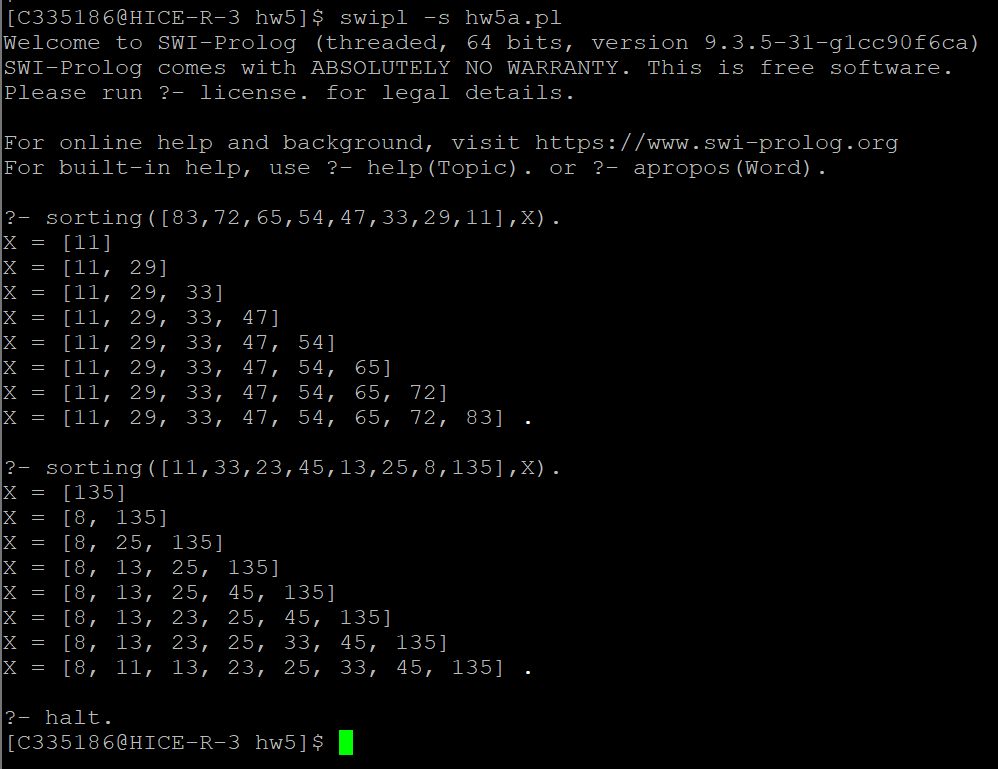
\includegraphics[width=1\linewidth]{결과1.png}
    \caption{hw5a.pl 결과}
    \label{fig:enter-label}
\end{figure}



\newpage
\section{hw5b.pl}
\subsection{hw5b.pl 코드}
\begin{lstlisting}

n_queen(N, X) :-
    numlist(1, N, Ns),       % Generate list [1, 2, ..., N]
    permutation(Ns, Sol),    % Try all possible row permutations
    safe_all(Sol),           % Check no diagonal conflicts
    reverse(Sol, X),         % Reverse solution for final output
    !.                       % Commit to first solution and prevent backtracking

% safe_all(List): Succeeds if no two queens in List attack diagonally
safe_all([]).               % Empty list: no conflicts
safe_all([H|T]) :-
    safe(H, T, 1),           % Check head H against the rest with initial diagonal distance 1
    safe_all(T).             % Then check remaining queens recursively

% safe(Row, Rows, D): Succeeds if Row does not conflict with any in Rows at diagonal distance D
% Row: Row position of the current queen
% Rows: Remaining row positions to check against
% D: Current column distance from the queen at Row
safe(_, [], _).             % No more queens to compare: safe
safe(R, [R1|Rs], D) :-
    R =\= R1 + D,            % Not on downward-right diagonal
    R =\= R1 - D,            % Not on upward-right diagonal
    D1 is D + 1,             % Increase diagonal distance for the next queen
    safe(R, Rs, D1).         % Recurse on remaining queens



\end{lstlisting}

\subsection{hw5b.pl 코드 설명 (trace 사용)}

길이가 길기 때문에 가독성을 위해 따로 캡쳐 없어 trace를 전부 복사해왔다. n=3 인 경우로 예시를 들어보았다.  

\begin{lstlisting}
?- trace.
true.

[trace]  ?- n_queen(3,X).
   Call: (12) n_queen(3, _4822) ? creep
   Call: (13) lists:numlist(1, 3, _6120) ? creep
   Exit: (13) lists:numlist(1, 3, [1, 2, 3]) ? creep
   Call: (13) lists:permutation([1, 2, 3], _13268) ? creep
   Exit: (13) lists:permutation([1, 2, 3], [1, 2, 3]) ? creep
   Call: (13) safe_all([1, 2, 3]) ? creep
   Call: (14) safe(1, [2, 3], 1) ? creep
   Call: (15) 1=\=2+1 ? creep
   Exit: (15) 1=\=2+1 ? creep
   Call: (15) 1=\=2-1 ? creep
   Fail: (15) 1=\=2-1 ? creep
   Fail: (14) safe(1, [2, 3], 1) ? creep
   Fail: (13) safe_all([1, 2, 3]) ? creep
   Redo: (13) lists:permutation([1, 2, 3], [1, 2, 3]) ? creep
   Exit: (13) lists:permutation([1, 2, 3], [1, 3, 2]) ? creep
   Call: (13) safe_all([1, 3, 2]) ? creep
   Call: (14) safe(1, [3, 2], 1) ? creep
   Call: (15) 1=\=3+1 ? creep
   Exit: (15) 1=\=3+1 ? creep
   Call: (15) 1=\=3-1 ? creep
   Exit: (15) 1=\=3-1 ? creep
   Call: (15) _28208 is 1+1 ? creep
   Exit: (15) 2 is 1+1 ? creep
   Call: (15) safe(1, [2], 2) ? creep
   Call: (16) 1=\=2+2 ? creep
   Exit: (16) 1=\=2+2 ? creep
   Call: (16) 1=\=2-2 ? creep
   Exit: (16) 1=\=2-2 ? creep
   Call: (16) _33902 is 2+1 ? creep
   Exit: (16) 3 is 2+1 ? creep
   Call: (16) safe(1, [], 3) ? creep
   Exit: (16) safe(1, [], 3) ? creep
   Exit: (15) safe(1, [2], 2) ? creep
   Exit: (14) safe(1, [3, 2], 1) ? creep
   Call: (14) safe_all([3, 2]) ? creep
   Call: (15) safe(3, [2], 1) ? creep
   Call: (16) 3=\=2+1 ? creep
   Fail: (16) 3=\=2+1 ? creep
   Fail: (15) safe(3, [2], 1) ? creep
   Fail: (14) safe_all([3, 2]) ? creep
   Redo: (16) safe(1, [], 3) ? creep
   Fail: (16) safe(1, [], 3) ? creep
   Fail: (15) safe(1, [2], 2) ? creep
   Fail: (14) safe(1, [3, 2], 1) ? creep
   Fail: (13) safe_all([1, 3, 2]) ? creep
   Redo: (13) lists:permutation([1, 2, 3], [1, 3, 2]) ? creep
   Exit: (13) lists:permutation([1, 2, 3], [2, 1, 3]) ? creep
   Call: (13) safe_all([2, 1, 3]) ? creep
   Call: (14) safe(2, [1, 3], 1) ? creep
   Call: (15) 2=\=1+1 ? creep
   Fail: (15) 2=\=1+1 ? creep
   Fail: (14) safe(2, [1, 3], 1) ? creep
   Fail: (13) safe_all([2, 1, 3]) ? creep
   Redo: (13) lists:permutation([1, 2, 3], [2, 1, 3]) ? creep
   Exit: (13) lists:permutation([1, 2, 3], [2, 3, 1]) ? creep
   Call: (13) safe_all([2, 3, 1]) ? creep
   Call: (14) safe(2, [3, 1], 1) ? creep
   Call: (15) 2=\=3+1 ? creep
   Exit: (15) 2=\=3+1 ? creep
   Call: (15) 2=\=3-1 ? creep
   Fail: (15) 2=\=3-1 ? creep
   Fail: (14) safe(2, [3, 1], 1) ? creep
   Fail: (13) safe_all([2, 3, 1]) ? creep
   Redo: (13) lists:permutation([1, 2, 3], [2, 3, 1]) ? creep
   Exit: (13) lists:permutation([1, 2, 3], [3, 1, 2]) ? creep
   Call: (13) safe_all([3, 1, 2]) ? creep
   Call: (14) safe(3, [1, 2], 1) ? creep
   Call: (15) 3=\=1+1 ? creep
   Exit: (15) 3=\=1+1 ? creep
   Call: (15) 3=\=1-1 ? creep
   Exit: (15) 3=\=1-1 ? creep
   Call: (15) _3954 is 1+1 ? creep
   Exit: (15) 2 is 1+1 ? creep
   Call: (15) safe(3, [2], 2) ? creep
   Call: (16) 3=\=2+2 ? creep
   Exit: (16) 3=\=2+2 ? creep
   Call: (16) 3=\=2-2 ? creep
   Exit: (16) 3=\=2-2 ? creep
   Call: (16) _9648 is 2+1 ? creep
   Exit: (16) 3 is 2+1 ? creep
   Call: (16) safe(3, [], 3) ? creep
   Exit: (16) safe(3, [], 3) ? creep
   Exit: (15) safe(3, [2], 2) ? creep
   Exit: (14) safe(3, [1, 2], 1) ? creep
   Call: (14) safe_all([1, 2]) ? creep
   Call: (15) safe(1, [2], 1) ? creep
   Call: (16) 1=\=2+1 ? creep
   Exit: (16) 1=\=2+1 ? creep
   Call: (16) 1=\=2-1 ? creep
   Fail: (16) 1=\=2-1 ? creep
   Fail: (15) safe(1, [2], 1) ? creep
   Fail: (14) safe_all([1, 2]) ? creep
   Redo: (16) safe(3, [], 3) ? creep
   Fail: (16) safe(3, [], 3) ? creep
   Fail: (15) safe(3, [2], 2) ? creep
   Fail: (14) safe(3, [1, 2], 1) ? creep
   Fail: (13) safe_all([3, 1, 2]) ? creep
   Redo: (13) lists:permutation([1, 2, 3], [3, 1, 2]) ? creep
   Exit: (13) lists:permutation([1, 2, 3], [3, 2, 1]) ? creep
   Call: (13) safe_all([3, 2, 1]) ? creep
   Call: (14) safe(3, [2, 1], 1) ? creep
   Call: (15) 3=\=2+1 ? creep
   Fail: (15) 3=\=2+1 ? creep
   Fail: (14) safe(3, [2, 1], 1) ? creep
   Fail: (13) safe_all([3, 2, 1]) ? creep
   Redo: (13) lists:permutation([1, 2, 3], [3, 2, 1]) ? creep
   Fail: (13) lists:permutation([1, 2, 3], _136) ? creep
   Fail: (12) n_queen(3, _58) ? creep
false.

[trace]  ?-

\end{lstlisting}

위 trace를 보고 구조를 파악해보자.  

\\ \\

\begin{enumerate}

\item
\begin{verbatim}
Call: (12) n_queen(3, _4822) ? creep
\end{verbatim}
n\_queen(3, \_4822)가 호출된다. N=3짜리 문제를 해결해보자.

\item
\begin{verbatim}
Call: (13) lists:numlist(1, 3, _6120) ? creep
Exit: (13) lists:numlist(1, 3, [1, 2, 3]) ? creep
\end{verbatim}
lists:numlist를 통해 [1,2,3] 리스트를 만든다. 이 리스트는 가능한 열 번호들을 나타낸다.

\item
\begin{verbatim}
Call: (13) lists:permutation([1, 2, 3], _13268) ? creep
Exit: (13) lists:permutation([1, 2, 3], [1, 2, 3]) ? creep
Call: (13) safe_all([1, 2, 3]) ? creep
\end{verbatim}
첫 번째 배열 [1,2,3]에 대해 safe\_all 검사를 시작한다.

\item
\begin{verbatim}
Call: (14) safe(1, [2, 3], 1) ? creep
Call: (15) 1=\=2+1 ? creep
Exit: (15) 1=\=2+1 ? creep
Call: (15) 1=\=2-1 ? creep
Fail: (15) 1=\=2-1 ? creep
\end{verbatim}
두 번째 퀸(2행 2열)이 대각선 위에 위치하므로 충돌 발생이므로 실패.

\item
\begin{verbatim}
Fail: (14) safe(1, [2, 3], 1) ? creep
Fail: (13) safe_all([1, 2, 3]) ? creep
\end{verbatim}
이 배열은 불가능한 배치로 판단된다.

\item
\begin{verbatim}
Redo: (13) lists:permutation([1, 2, 3], [1, 2, 3]) ? creep
Exit: (13) lists:permutation([1, 2, 3], [1, 3, 2]) ? creep
Call: (13) safe_all([1, 3, 2]) ? creep
\end{verbatim}
다음 배배열 [1,3,2]로 넘어가 검사를 시작한다.

\item
\begin{verbatim}
Call: (14) safe(1, [3, 2], 1) ? creep
Call: (15) 1=\=3+1 ? creep
Exit: (15) 1=\=3+1 ? creep
Call: (15) 1=\=3-1 ? creep
Exit: (15) 1=\=3-1 ? creep
\end{verbatim}
두 번째 퀸(2행 3열)과 충돌 없음. 다음 퀸 검사로 진행.

\item
\begin{verbatim}
Call: (15) safe(1, [2], 2) ? creep
Call: (16) 1=\=2+2 ? creep
Exit: (16) 1=\=2+2 ? creep
Call: (16) 1=\=2-2 ? creep
Exit: (16) 1=\=2-2 ? creep
\end{verbatim}
세 번째 퀸(3행 2열)도 대각선 충돌이 없다.

\item
\begin{verbatim}
Exit: (16) safe(1, [], 3) ? creep
Exit: (15) safe(1, [2], 2) ? creep
Exit: (14) safe(1, [3, 2], 1) ? creep
\end{verbatim}
현재까지 [1,3,2]는 모두 안전하게 배치된다.

\item
\begin{verbatim}
Call: (14) safe_all([3, 2]) ? creep
Call: (15) safe(3, [2], 1) ? creep
Call: (16) 3=\=2+1 ? creep
Fail: (16) 3=\=2+1 ? creep
\end{verbatim}
[3,2] 부분에서 2행 퀸과 3행 퀸이 대각선 충돌이므로 실패.

\item
\begin{verbatim}
Fail: (14) safe_all([3, 2]) ? creep
Fail: (13) safe_all([1, 3, 2]) ? creep
\end{verbatim}
[1,3,2]도 결국 불가능 판정.

\item
이후 배열 [2,1,3], [2,3,1], [3,1,2], [3,2,1]에 대해 같은 방식으로 permutation과 safe\_all, safe가 반복 호출된다.  
각 배열마다 대각선 충돌이 발생하여 모두 실패로 처리된다.

\item
\begin{verbatim}
Fail: (12) n_queen(3, _58) ? creep
false.
\end{verbatim}
모든 배열이 실패했으므로 N=3은 해가 없다고 판정되어 false가 반환된다. \\ \\

\end{enumerate}


이렇게 간단한 예시로 구조를 살펴보았다. 다시한번 정리하자면 \\ \\
\texttt{->} \texttt{n\_queen(3, X)} 호출 시, \texttt{numlist}를 통해 \texttt{[1, 2, 3]} 리스트를 생성한다. \\
\texttt{->} 생성된 리스트의 모든 \texttt{permutation}을 시도하며 배열을 하나씩 만든다.\\
\texttt{->} 각 배열마다 \texttt{safe\_all}를 호출하여 대각선 충돌 여부를 검사한다. \\
\texttt{->} 충돌이 발생하면 실패하고, backtracking을 통해 다음 배열을 시도한다. \\
\texttt{->} N=3에서는 모든 배열에서 충돌이 발생하여 결국 \texttt{false}를 반환한다. \\


이런 구조이다.


\subsection{hw5b.pl 실행 결과}

\begin{figure} [H]
    \centering
    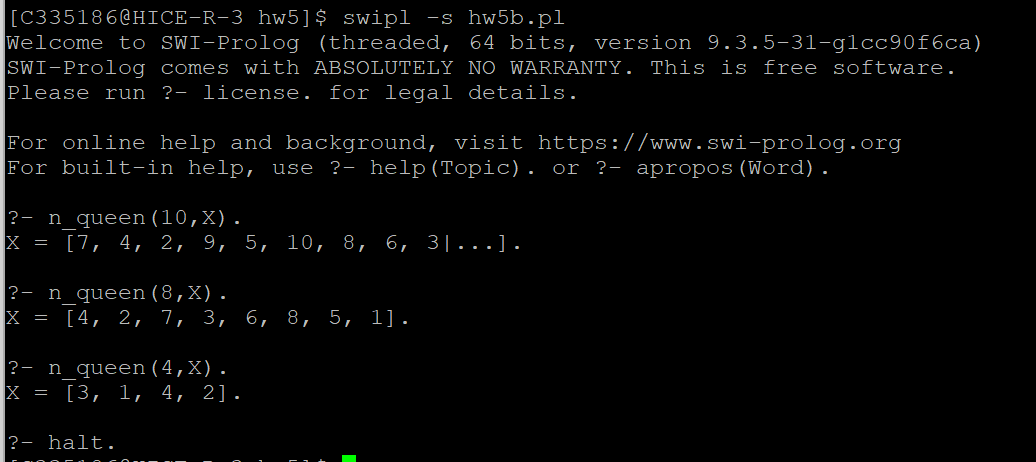
\includegraphics[width=1\linewidth]{결과2.png}
    \caption{Enter Caption}
    \label{fig:enter-label}
\end{figure}





\end{document}

